\begin{problem}{수상자 수 결정하기}{standard input}{standard output}{4 seconds}{1024 megabytes}

오늘 A 학교에서 $1$번부터 $N$번까지 번호가 매겨진 $N$명의 학생이 $100$미터 달리기 경주를 하려고 합니다.

이때 여러분은 다음과 같은 정보를 총 $M$개 알고 있습니다.

\begin{itemize}
\item $i$ $j$: $i$번 학생과 $j$번 학생이 달리기 경주를 할 경우, 항상 $i$번 학생이 결승선에 먼저 들어옵니다.
\end{itemize}

단, 여러분의 정보는 언제나 정확하기 때문에, 모순되는 정보는 주어지지 않습니다. 또한, 어떤 두 학생을 골라도 기록이 서로 같지 않습니다.

여러분은 이 $N$명의 학생이 달리기 경주를 했을 때 결승선에 가장 먼저 들어온 $K$명에게 상을 주려고 합니다. 그러던 중 여러분은 다음과 같은 고민에 빠졌습니다.

\begin{itemize}
\item 학생들의 기록이 어떻게 결정되어도 가장 먼저 들어온 $K$명의 집합이 항상 동일하다면, 달리기 경주가 재미없게 됩니다.
\end{itemize}

예를 들어, $4$명의 학생이 있고 그 관계가 다음과 같다고 생각합시다. $i$에서 $j$로 향하는 화살표는 $i$번 학생이 항상 $j$번 학생보다 먼저 들어옴을 의미합니다.

\begin{center}
  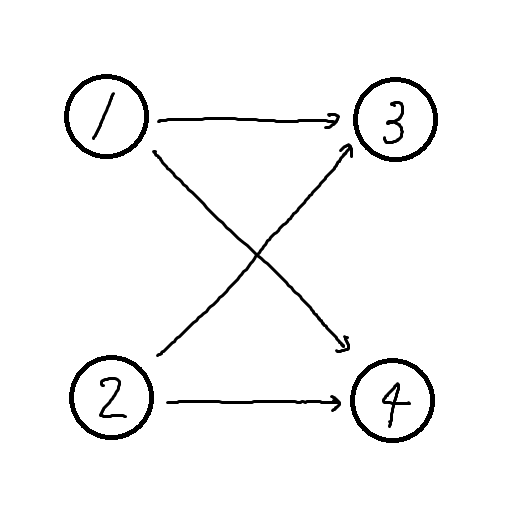
\includegraphics[scale=0.5]{winnerset.png}
\end{center}

이때 $K=2$라면 가장 먼저 들어온 $2$명은 항상 $1$번 학생과 $2$번 학생이므로 달리기 경주가 재미없게 됩니다.

$K=1,2,\ldots,N$에 대해 각각, $K$명에게 상을 줄 때 달리기 경주가 재미없게 되는지 구하는 프로그램을 작성해 주세요.

\InputFile
첫 번째 줄에 테스트 케이스의 개수 $T$가 주어집니다.

그다음 줄부터 $T$개의 테스트 케이스가 주어집니다. 테스트 케이스의 형식은 다음과 같습니다.

첫 번째 줄에는 두 정수 $N$과 $M$이 공백으로 구분되어 주어집니다.

두 번째 줄부터 $M$개의 줄에 걸쳐 각각 정보를 나타내는 두 정수 $i_k$와 $j_k$가 주어집니다.

\OutputFile
각 테스트 케이스에 대해 길이 $N$의 문자열 $S$를 새로운 줄에 출력합니다. 이때 $S$는 다음과 같이 정의됩니다.

\begin{itemize}
\item $K=i$일 때 경주가 재미없게 된다면 $S_i$는 `\texttt{1}'입니다.
\item $K=i$일 때 경주가 재미없게 되지 않는다면 $S_i$는 `\texttt{0}'입니다.
\end{itemize}

\Scoring
\begin{itemize}
\item $1 \le T \le 1000$
\item $2 \le N \le 300\,000$
\item $1 \le M \le 500\,000$
\item 모든 테스트 케이스에서 $N$의 합은 $300\,000$을 초과하지 않습니다.
\item 모든 테스트 케이스에서 $M$의 합은 $500\,000$을 초과하지 않습니다.
\item 주어진 $M$개의 정보는 항상 서로 다릅니다.
\item 주어진 $M$개의 정보는 모순되지 않습니다.
\end{itemize}

\textbf{서브태스크}

\begin{tabular}{|l|l|l|} \hline
  \textbf{번호} & \textbf{배점} & \textbf{제한} \\ \hline
  1 & 11 & $N$의 합은 $10$ 이하 \\ \hline
  2 & 13 & $N$의 합은 $20$ 이하 \\ \hline
  3 & 17 & $N$의 합은 $200$ 이하 \\ \hline
  4 & 21 & $N$의 합은 $2000$ 이하, $M$의 합은 $20\,000$ 이하 \\ \hline
  5 & 38 & 추가 제한 없음 \\ \hline
\end{tabular}

\Example

\begin{example}
\exmpfile{example.01}{example.01.a}%
\end{example}

\Note
첫 번째 테스트 케이스는 지문에 주어진 그림과 같습니다.

두 번째 테스트 케이스에서 $4$명의 학생에 대해 알고 있는 정보는 다음과 같습니다.

\begin{itemize}
\item $1$번 학생은 $2$번 학생보다 항상 먼저 들어옵니다.
\item $1$번 학생은 $3$번 학생보다 항상 먼저 들어옵니다.
\item $3$번 학생은 $4$번 학생보다 항상 먼저 들어옵니다. 
\end{itemize}

이때 각 $K$의 값에 대한 설명은 다음과 같습니다.

\begin{itemize}
\item $K=1$일 때 가장 먼저 들어온 학생은 항상 $1$번 학생입니다.
\item $K=2$일 때 가장 먼저 들어온 $2$명의 집합은 $\{1,2\}$ 또는 $\{1,3\}$입니다.
\item $K=3$일 때 가장 먼저 들어온 $3$명의 집합은 $\{1,2,3\}$ 또는 $\{1,3,4\}$입니다.
\item $K=4$일 때 가장 먼저 들어온 $4$명의 집합은 $\{1,2,3,4\}$입니다.
\end{itemize}

그러므로 $K=1$ 또는 $K=4$일 때 달리기 경주가 재미없게 됩니다.

\end{problem}

